\newpage
\chapter{Discussion and Conclusion}
\label{sec:Discussion}

\begin{wrapfigure}{r}{6cm}
    \centering
    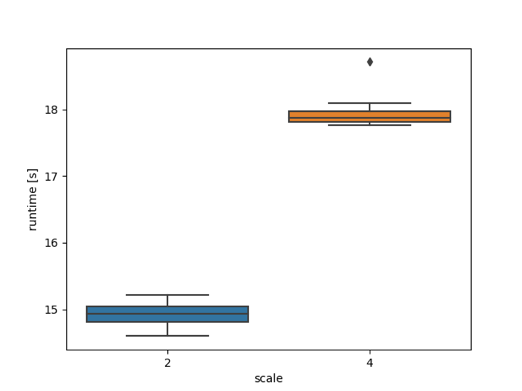
\includegraphics[width=6cm]{figures/aetad_very_small_runtime.png}
    \caption{Runtime on Mac Pro 2015 for one scaling operation using \textit{aetad\_very\_small} in comparison to 37s (x2) / 51s (x4) using baseline model.}
    \label{fig:aetad_very_small_runtime}
\end{wrapfigure}

The goals of this work were to improve the performance-runtime tradeoff of task aware downscaling for the single-image super-resolution problem and image colorization problem, to increase the robustness against perturbations and to extend it to the video domain, shown based on the video super-resolution task.
\newline
As largely presented in \mysecref{sec:ExperimentsandResults} more reasonable models could be found by adaptions of both the model architecture and the training procedure. Thus, for the \ac{SISR} problem a model could be derived with slightly worse (but mostly similar) performance but
$44 \%$ less model parameters, compared to the baseline architecture by Kim et al. \cite{TAID}, which highly decreases the model's runtime on non-GPU hardware (from $51s$ to about $18s$ for a single forward pass with scaling factor $4$ on a Mac Pro 2015, comp. \myfigref{fig:aetad_very_small_runtime}). Also for the \ac{IC} task a more reasonable model was derived. Due to the reconstruction performance peaking with a slight increase of the model's complexity, the final model is larger, but increases reconstruction accuracy by $31 \%$. Likewise a method to improve robustness against perturbation and performance ($\epsilon = 1$) as well as the trade-off between reconstruction performance with and without perturbation was demonstrated. As shown introducing \ac{TAD} to the video domain by training an external \ac{VSR} model (here Wang et al. \cite{LFVSRTHROFE}) improves its reconstruction accuracy on every validation dataset used. Overall the \ac{TAD} purposed by Kim et al. was thus widely improved and extended within this work. 
\newline 
In general \ac{TAD} can improve the reconstruction performance both quantitatively in terms of \ac{PSNR} as well as qualitatively in terms of enabling reconstruction of otherwise irreconstrucable images, while being very efficient compared to other state-of-the-art models (in terms of model complexity, e.g. compared to \myfigref{fig:vdsr} having 20 layers for upscaling only). However, it comes at the price of computational cost, as it is clearly more expensive than trivial downscaling methods such as averaging over channels or bilinear/bicubic interpolation. Nevertheless this work contributed to a more efficient way of task aware downscaling there still is some work to do in order to further compress the models used to make them practicable on non-GPU devices such as mobile phones, so that it can be used as alternative of bilinear compression e.g. in messenger or mailing services. Also the underlying project demonstrated the feasibility of applying \ac{TAD} on the video domain for the \ac{VSR} problem combined with a scaling factor up to $4$. Further work could integrate other external models as well as use examine the performance for larger scaling factors such as $16$. Furthermore during this work it was assumed to have a constant compression rate while improving the reconstruction performance. Although the model already outperforms standard compression algorithms such as jpeg further work can be done to meet both the readability constraint of the low-dimensional image as well as a more dense representation of the high-dimensional data. The \ac{TAD} architecture used within is very much constrained on the size on the size of the guidance image, although there might be a more dense representation of the high-dimensional data (due to the readability constraint). However, a double autoencoder structure as displayed in \myfigref{fig:future_work_double_tad} could resolve the problem, by first downscale to a human understandable representation and then further compress to a more dense representation. Thereby, to avoid interdependent optimization therefore the outer autoencoder could be fixed while training the inner autoencoder. 

\begin{figure}[!htbp]
	\centering
	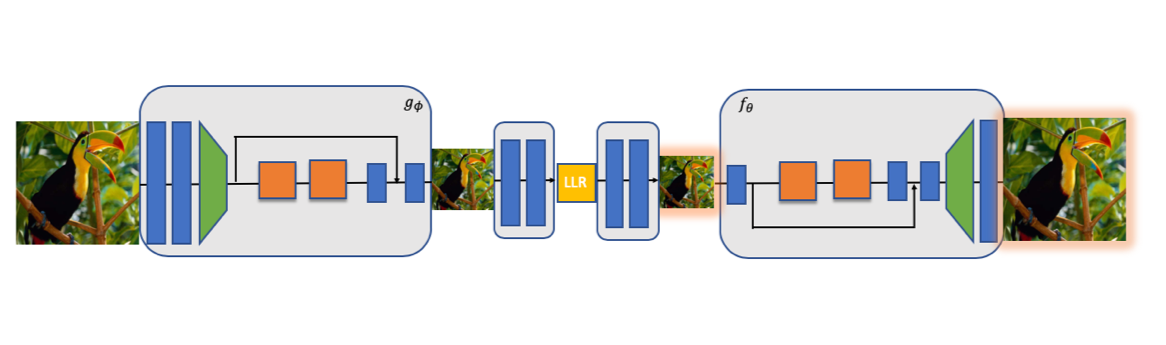
\includegraphics[width=16cm]{figures/future_work_double_tad.png}
	\caption{Double \ac{TAD} architecture for improvement in compression rate.}
  \label{fig:future_work_double_tad}
\end{figure}

% The discussion section gives an interpretation of what you have done :
%
% \begin{itemize}
%  \item \textit{What do your results mean?} Here you discuss, but you do not recapitulate results. Describe principles, relationships and generalizations shown. Also, mention inconsistencies or exceptions you found.
%  \item \textit{How do your results relate to other's work?} Show how your work agrees or disagrees with other's work. Here you can rely on the information you presented in the ``related work'' section.
%  \item \textit{What are implications and applications of your work?} State how your methods may be applied and what implications might be.
% \end{itemize}
%
% \noindent Make sure that introduction/related work and the discussion section act as a pair, i.e. ``be sure the discussion section answers what the introduction section asked'' .

% List the conclusions of your work and give evidence for these.

